\documentclass[12pt, notitlepage, final]{article} 

\newcommand{\name}{Vince Coghlan}

\usepackage{amsfonts}
\usepackage{amssymb}
\usepackage{amsmath}
\usepackage{latexsym}
\usepackage{enumerate}
\usepackage{amsthm}
\usepackage{nccmath}
\usepackage{setspace}
\usepackage[pdftex]{graphicx}
\usepackage{epstopdf}
\usepackage[siunitx]{circuitikz}
\usepackage{tikz}
\usepackage{float}
\usepackage{cancel}
\usepackage{pgfplots}
\usepackage{setspace}
\usepackage{overpic}
\usepackage{mathtools}
\usepackage{listings}
\usepackage{color}

\numberwithin{equation}{section}
\DeclareRobustCommand{\beginProtected}[1]{\begin{#1}}
\DeclareRobustCommand{\endProtected}[1]{\end{#1}}
\newcommand{\dbr}[1]{d_{\mbox{#1BR}}}
\newtheorem{lemma}{Lemma}
\newtheorem*{corollary}{Corollary}
\newtheorem{theorem}{Theorem}
\newtheorem{proposition}{Proposition}
\theoremstyle{definition}
\newtheorem{define}{Definition}
\newcommand{\column}[2]{
\left( \begin{array}{ccc}
#1 \\
#2
\end{array} \right)}

\newdimen\digitwidth
\settowidth\digitwidth{0}
\def~{\hspace{\digitwidth}}

\setlength{\parskip}{1pc}
\setlength{\parindent}{0pt}
\setlength{\topmargin}{-3pc}
\setlength{\textheight}{9.0in}
\setlength{\oddsidemargin}{0pc}
\setlength{\evensidemargin}{0pc}
\setlength{\textwidth}{6.5in}
\newcommand{\answer}[1]{\newpage\noindent\framebox{\vbox{{\bf ECEN 4610
      \hfill {\bf Capstone Fall 2014}} \vspace{-0.7cm}
\begin{center}{The League of Extraordinary Engineers Team\\Responsibilities and System Diagram}\end{center} } }\bigskip }
\newcommand{\answertwo}[1]{\newpage\noindent\framebox{\vbox{{\bf ECEN 4610
      \hfill {\bf Capstone Fall 2014}} \vspace{-0.7cm}
\begin{center}{The League of Extraordinary Engineers Team\\Functional Decomposition}\end{center} } }\bigskip }
%absolute value code
\DeclarePairedDelimiter\abs{\lvert}{\rvert}%
\DeclarePairedDelimiter\norm{\lVert}{\rVert}
\makeatletter
\let\oldabs\abs
\def\abs{\@ifstar{\oldabs}{\oldabs*}}
%
\let\oldnorm\norm
\def\norm{\@ifstar{\oldnorm}{\oldnorm*}}
\makeatother

\def\dbar{{\mathchar'26\mkern-12mu d}}
\def \Frac{\displaystyle\frac}
\def \Sum{\displaystyle\sum}
\def \Int{\displaystyle\int}
\def \Prod{\displaystyle\prod}
\def \P[x]{\Frac{\partial}{\partial x}}
\def \D[x]{\Frac{d}{dx}}
\newcommand{\PD}[2]{\frac{\partial#1}{\partial#2}}
\newcommand{\PF}[1]{\frac{\partial}{\partial#1}}
\newcommand{\DD}[2]{\frac{d#1}{d#2}}
\newcommand{\DF}[1]{\frac{d}{d#1}}
\newcommand{\fix}[2]{\left(#1\right)_#2}
\newcommand{\ket}[1]{|#1\rangle}
\newcommand{\bra}[1]{\langle#1|}
\newcommand{\braket}[2]{\langle #1 | #2 \rangle}
\newcommand{\bopk}[3]{\langle #1 | #2 | #3 \rangle}
\newcommand{\Choose}[2]{\displaystyle {#1 \choose #2}}
\newcommand{\proj}[1]{\ket{#1}\bra{#1}}
\def\del{\vec{\nabla}}
\newcommand{\avg}[1]{\langle#1\rangle}
\newcommand{\piecewise}[4]{\left\{\beginProtected{array}{rl}#1&:#2\\#3&:#4\endProtected{array}\right.}
\newcommand{\systeme}[2]{\left\{\beginProtected{array}{rl}#1\\#2\endProtected{array}\right.}
\def \KE{K\!E}
\def\Godel{G$\ddot{\mbox{o}}$del}

\onehalfspacing

\begin{document}

\answer{}
\begin{center}
  \begin{tabular}{ | p{4cm} | p{3cm} | p{4cm} | p{4cm} |}
    \hline
    Responsibilities & Roles & Hardware & Software \\ \hline \hline
    Trigger Capacitor Plates When Car is Above & MotherBrain & Decoder and control bus & Plate Control Logic \\ \hline
    Sense Car & RFID & RFID transmitter and reciever & RFID Controls on Vehicle \\ \hline
    Transmit Power & Road Power & Freq Converter, plates, and connection to power grid & - \\ \hline
    Recieve Power & Vehicle Power & Rectifier/Converter, battery, plates, and motors & - \\
    \hline
    \end{tabular}
\end{center}

\begin{figure}[H]
\begin{center}
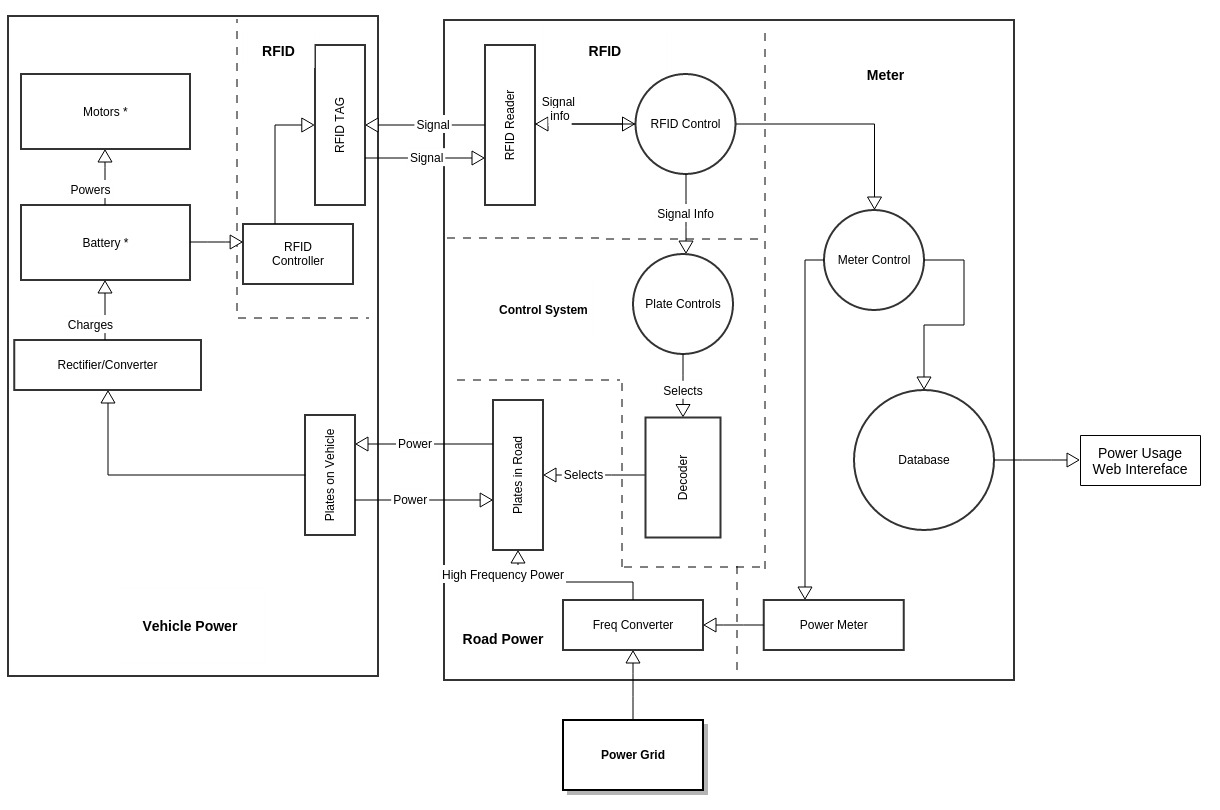
\includegraphics[width=14cm]{sd}
\end{center}
\end{figure}

\newpage
\answertwo

\section{Function Decomposition Level 0 - Part 1}
\begin{center}
  \begin{tabular}{ | p{3cm} | p{8cm} |}
    \hline
    Module & Onboard Vehicle Power System \\ \hline \hline
    Inputs & Wireless energy from chargin pads \\
     & Battery Voltage Levels \\ \hline
    Outputs & RFID Signal \\
     & DC power to battery \\ \hline
    Functionality & The onboard system will take in battery voltafe levels to
    determine if the battery needs to acquire power from the road.  Based on this information,
    differenct codes will be transmitted by the vehicle RFID tag in order to
    request power when needed. The onboard system the recieves power transmitted
    by the charge pads in the road power system and outputs the received energy
    in order to charge the vehicle battery. \\
    \hline
    \end{tabular}
\end{center}

\begin{figure}[H]
\begin{center}
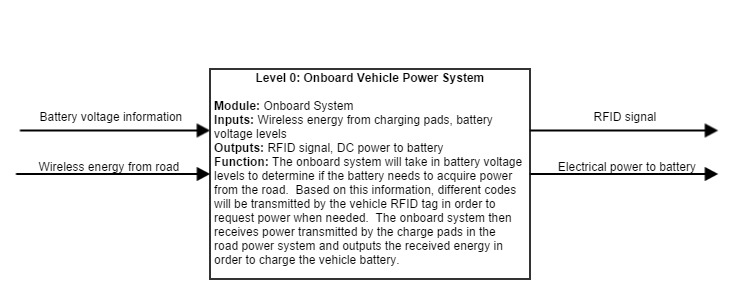
\includegraphics[width=14cm]{func_decomp_lvl_0}
\end{center}
\end{figure}

\section{Functional Decomposition Level 0 - Part 2}
\begin{center}
  \begin{tabular}{ | p{3cm} | p{8cm} |}
    \hline
    Module & Road Surface Power System \\ \hline \hline
    Inputs & RFID signal \\
     & 120V/60Hz Electrical Power \\ \hline
    Outputs & ISM-Band Wireless Power \\
     & Power Metering Information \\ \hline
    Functionality & The road surface power system is powered by mains
    power from the electrical grid.  An RFID reader and control
    subsystem determines if power should be transmitted, based on the
    input RFID signal.  Based on RFID readings the proper road-surface level
    charge pads are place in power transmit mode and output wireless power in an
    ISM band.  The road system also meters power used by each vehicle and
    stores it in a database to be accesed on the web by users or power companies\\
    \hline
    \end{tabular}
\end{center}


\begin{figure}[H]
\begin{center}
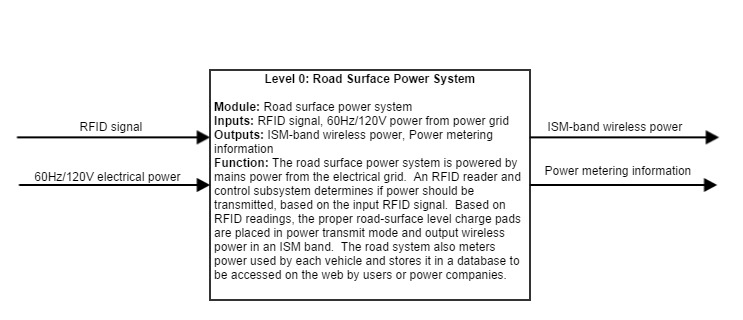
\includegraphics[width=14cm]{func_decomp_lvl_0_part2}
\end{center}
\end{figure}

\section{Function Decomposition Level 1 - Part 1}

\subsection{Road Modules}
\begin{center}
  \begin{tabular}{| p{3cm} | p{8cm} |}
    \hline
    Module & Power Meter \\ \hline \hline
    Inputs & Power from the Power Grid \\ \hline
    Output & Electricity to the Frequency Converter and meter information to the meter controller \\ \hline
    Functionality & Reads the amount of power going into the system from the power grid \\ \hline
  \end{tabular}
\end{center}

\begin{center}
  \begin{tabular}{| p{3cm} | p{8cm} |}
    \hline
    Module & Frequency Converter \\ \hline \hline
    Inputs & 120V 60Hz AC power from power meter \\ \hline
    Output & Frequency Converted Signal to Capacitive Plates \\ \hline
    Functionality & Changes the frequency from that of the power grid \\ \hline
  \end{tabular}
\end{center}

\begin{center}
  \begin{tabular}{| p{3cm} | p{8cm} |}
    \hline
    Module & Capacitive Road Plates \\ \hline \hline
    Inputs & Frequency Converted Signal, Control Algorithm \\ \hline
    Output & Wireless Frequency Converted Signal, Metering Information \\ \hline
    Functionality & Enables conversion from normal signal over a wire to a
    wireless signal. There will be many of these that are turned on and off
    by the control algorithm from the control module. Outputs its on/off state
    to determine power usage. \\ \hline
  \end{tabular}
\end{center}

\begin{center}
  \begin{tabular}{| p{3cm} | p{8cm} |}
    \hline
    Module & RFID Reader \\ \hline \hline
    Inputs & RFID Signal from RFID Tag in Vehicle \\ \hline
    Output & Data to Control Module in Road and Metering Module \\ \hline
    Functionality & Reads the RFID tag in the vehicle to send data to the control and metering modules \\ \hline
  \end{tabular}
\end{center}

\begin{center}
  \begin{tabular}{| p{3cm} | p{8cm} |}
    \hline
    Module & Control Module \\ \hline \hline
    Inputs & RFID Reader Data \\ \hline
    Output & On/Off signal to Control the different road plates \\ \hline
    Functionality & This controls the Capacitive Road Plates. It determines if the capacitive plates need to be turned on based on the RFID data from the RFID Reader and turns them on and off \\ \hline
  \end{tabular}
\end{center}

\begin{center}
  \begin{tabular}{| p{3cm} | p{8cm} |}
    \hline
    Module & Metering Module \\ \hline \hline
    Inputs & Takes in data from the Power Meter and RFID Reader \\ \hline
    Output & Outputs data on power usage to a database \\ \hline
    Functionality & Is used to charge users for their power usage, by determining which vehicle is being charged through RFID data and how much power is being used from the power meter. \\ \hline
  \end{tabular}
\end{center}

\subsection{Vehicle Modules}

\begin{center}
  \begin{tabular}{| p{3cm} | p{8cm} |}
    \hline
    Module & Vehicle Capacitive Plate Module \\ \hline \hline
    Inputs & Wireless Power from the Road Capacitive Plates \\ \hline
    Output & Power over a wire to the Rectifier-Converter Module \\ \hline
    Functionality & Receives power capacitively from the roads Capacitive Plates Module and converts it to standard electricity over a wire \\ \hline
  \end{tabular}
\end{center}

\begin{center}
  \begin{tabular}{| p{3cm} | p{8cm} |}
    \hline
    Module & Rectifier-Converter Module \\ \hline \hline
    Inputs & Electricity from Vehicle Capacitive Plate Module \\ \hline
    Output & Rectified Electricity to Vehicle Battery \\ \hline
    Functionality & Converts the electricity from the capacitive plates to a current and voltage that can be used to charge the electric vehicles battery \\ \hline
  \end{tabular}
\end{center}

\begin{center}
  \begin{tabular}{| p{3cm} | p{8cm} |}
    \hline
    Module & RFID Controller \\ \hline \hline
    Inputs & Data regarding the batteries state \\ \hline
    Output & Control to the Active RFID Tag in the vehicle \\ \hline
    Functionality & Sends data to the RFID Tag in the vehicle. This data determines if the vehicle needs power from the Road. \\ \hline
  \end{tabular}
\end{center}

\begin{center}
  \begin{tabular}{| p{3cm} | p{8cm} |}
    \hline
    Module & Vehicle RFID Tag \\ \hline \hline
    Inputs & Data from RFID Controller\\ \hline
    Output & Wireless signal to the Road RFID Reader \\ \hline
    Functionality & Transmits the data from the RFID Controller to the RFID Reader in the Road. \\ \hline
  \end{tabular}
\end{center}


\end{document}
